\documentclass[11pt]{scrartcl}
\usepackage[utf8]{inputenc} % Kodierung der Textdatei mit Sonderzeichen
\usepackage[ngerman]{babel} % Sprache fuer Inhaltsverzeichnis etc.
\usepackage{amssymb} % Mathematische Symbole
\usepackage{amsmath} % Mehr mathematische Konstrukte
\usepackage{graphicx} % Um Bilder einbinden zu koennen
\usepackage{float} % fuer \begin{figure}[H]
\usepackage{icomma} % laesst das Komma als Dezimaltrennzeichen interpretieren
\usepackage{fix-cm} % für die große Titelschrift
\usepackage{placeins} % laesst Bilder nicht über eine \FloatBarrier hinausrutschen
\usepackage[pdftex]{hyperref} % Hyperlinks im Dokument
\hypersetup{colorlinks=true, linkcolor=black, citecolor=black, filecolor=black, urlcolor=black, pdftitle={LED-Spektrometer - Projektpraktikum 09/10 Gruppe 5}}


\newcommand{\unit}[1]{\ensuremath{\,\mathrm{#1}}} % Einheiten schreiben sich immer aufrecht!
\newcommand{\degr}{\ensuremath{^\circ}}
\newcommand{\cel}{\ensuremath{\degr\mathrm{C}}}
\newcommand{\dif}{\ensuremath{\mathrm{d}}}
\newcommand{\pdif}[2]{\ensuremath{\frac{\partial#1}{\partial#2}}}
\newcommand{\ee}[1]{\ensuremath{\cdot 10^{#1}}}
\newcommand{\hypref}[2]{\hyperref[#2]{{#1}~\ref{#2}}}

\setlength{\parindent}{1em}
\setlength{\parskip}{0.5\baselineskip}
\graphicspath{{images/}}


\title{LED-Spektrometer - Gruppe 5 WS 09/10, Projektpraktikum der Uni Erlangen}
\date{07.12.2009 -- 15.01.2010}
\author{Michele Collodo, Andreas Glossner, Karl-Christoph G\"odel, Bastian Hacker, Maria Obst, Alexander Wagner, David Winnekens}



\begin{document}
\sloppy % laesst Latex nicht ueber den Rand rausschreiben
\thispagestyle{empty}
\large{Projektpraktikum WS 09/10}
\hfill
\raisebox{-1.4cm}{
\includegraphics[width=5cm]{images/fau.pdf}}
\\[8\baselineskip]
\begin{center}
{\fontsize{36}{54}\textbf{LED-Spektrometer}}
\\[2\baselineskip]
{\Large 07.12.2009 -- 15.01.2010}
\\[7\baselineskip]
{\huge\textbf{PPG 5}}
\\[0.5\baselineskip]
{\large\textbf{
Michele Collodo,
Andreas Glossner,\\
Karl-Christoph G\"odel,
Bastian Hacker,\\
Maria Obst,
Alexander Wagner,
David Winnekens}\\
Tutor: Xiaoyue Jin}
\vfill



\small{\url{http://pp.physik.uni-erlangen.de/groups/ws0910/ppg5/ppg5\_start.html}}
\end{center}
\newpage



\tableofcontents
\vfill



\begin{abstract} %Andi
Verschiedenfarbige Leuchtdioden zeigen in der Absorption ihre größte Empfindlichkeit in einem zur Emissionswellenlänge leicht blauverschobenen Bereich. Ziel des Projekts war es nun, diesen in einer Vormessung nachgewiesenen Effekt zu nutzen, um ein Spektrometer aus verschiedenfarbigen LEDs zu konstruieren. 
Dabei wurden zunächst die Absorptionskurven verschiedener Leuchtdioden mit einem Gitterspektrum ermittelt. Anschließend diente eine Anordnung von 16 dieser LEDs als eigentliches Spektrometer. Das Spektrum einer unbekannten Lichtquelle im optischen Bereich konnte dann mit einer eigens entwickelten Auswertesoftware durch Entfaltung der Absorptionskurven ermittelt werden. Am Ende gelang es so, ein Spektrometer zu entwickeln, das vor allem bei Quellen mit glatten Spektren gute Resultate liefert. Gegenwärtig wird das Gerät unter Verwendung kleinerer SMD-Bauteile neu konstruiert und optimiert. 
\end{abstract}
\newpage

\section{Einleitung} %Andi
Spektrometer sind in verschiedensten Bereichen der Physik von hoher Bedeutung. Die Astronomie hat der Spektralanalyse weite Teile ihrer erzielten Durchbrüche zu verdanken und die Bedeutung von Spektren in der Optik muss nicht gesondert hervorgehoben werden. So finden heute  Spektrometer etwa im James Webb Space Telescope oder in der Röntgenastronomie Anwendung. Im Projekt war es nun das Ziel, ein solches für die Physik enorm bedeutsames Gerät zu konstruieren. Die Idee, dies unter Ausnutzung der unterschiedlichen Absorptionseigenschaften von verschiedenfarbigen Leuchtdioden zu versuchen, erschien schon aus einem sehr pragmatischen Grund vorteilhaft: Kommerziell wäre ein solches Gerät verhältnismäßig kostengünstig herzustellen, auch wenn der im Projekt verwendete Versuchsaufbau wohl eher dem Gegenwert eines Kleinwagens entspricht (bspw. empfindliche Spannungsmessgeräte für die Vormessungen, welche im serienreifen Spektrographen nicht mehr benötigt werden).



\section{Grundgedanke des Versuchs}
%% Allg. was wir machen wollen, etwas Theorie 	Karl


\subsection{Aufbau und Funktionsweise einer LED}
Die Leuchtdiode, kurz LED (für engl. "`Light Emitting Diode"') ist eine Halbleiter-Diode, die es ermöglicht elektrische Energie in Licht verschiedener Wellenlängen umzuwandeln.

\begin{figure}[ht]
\begin{center}
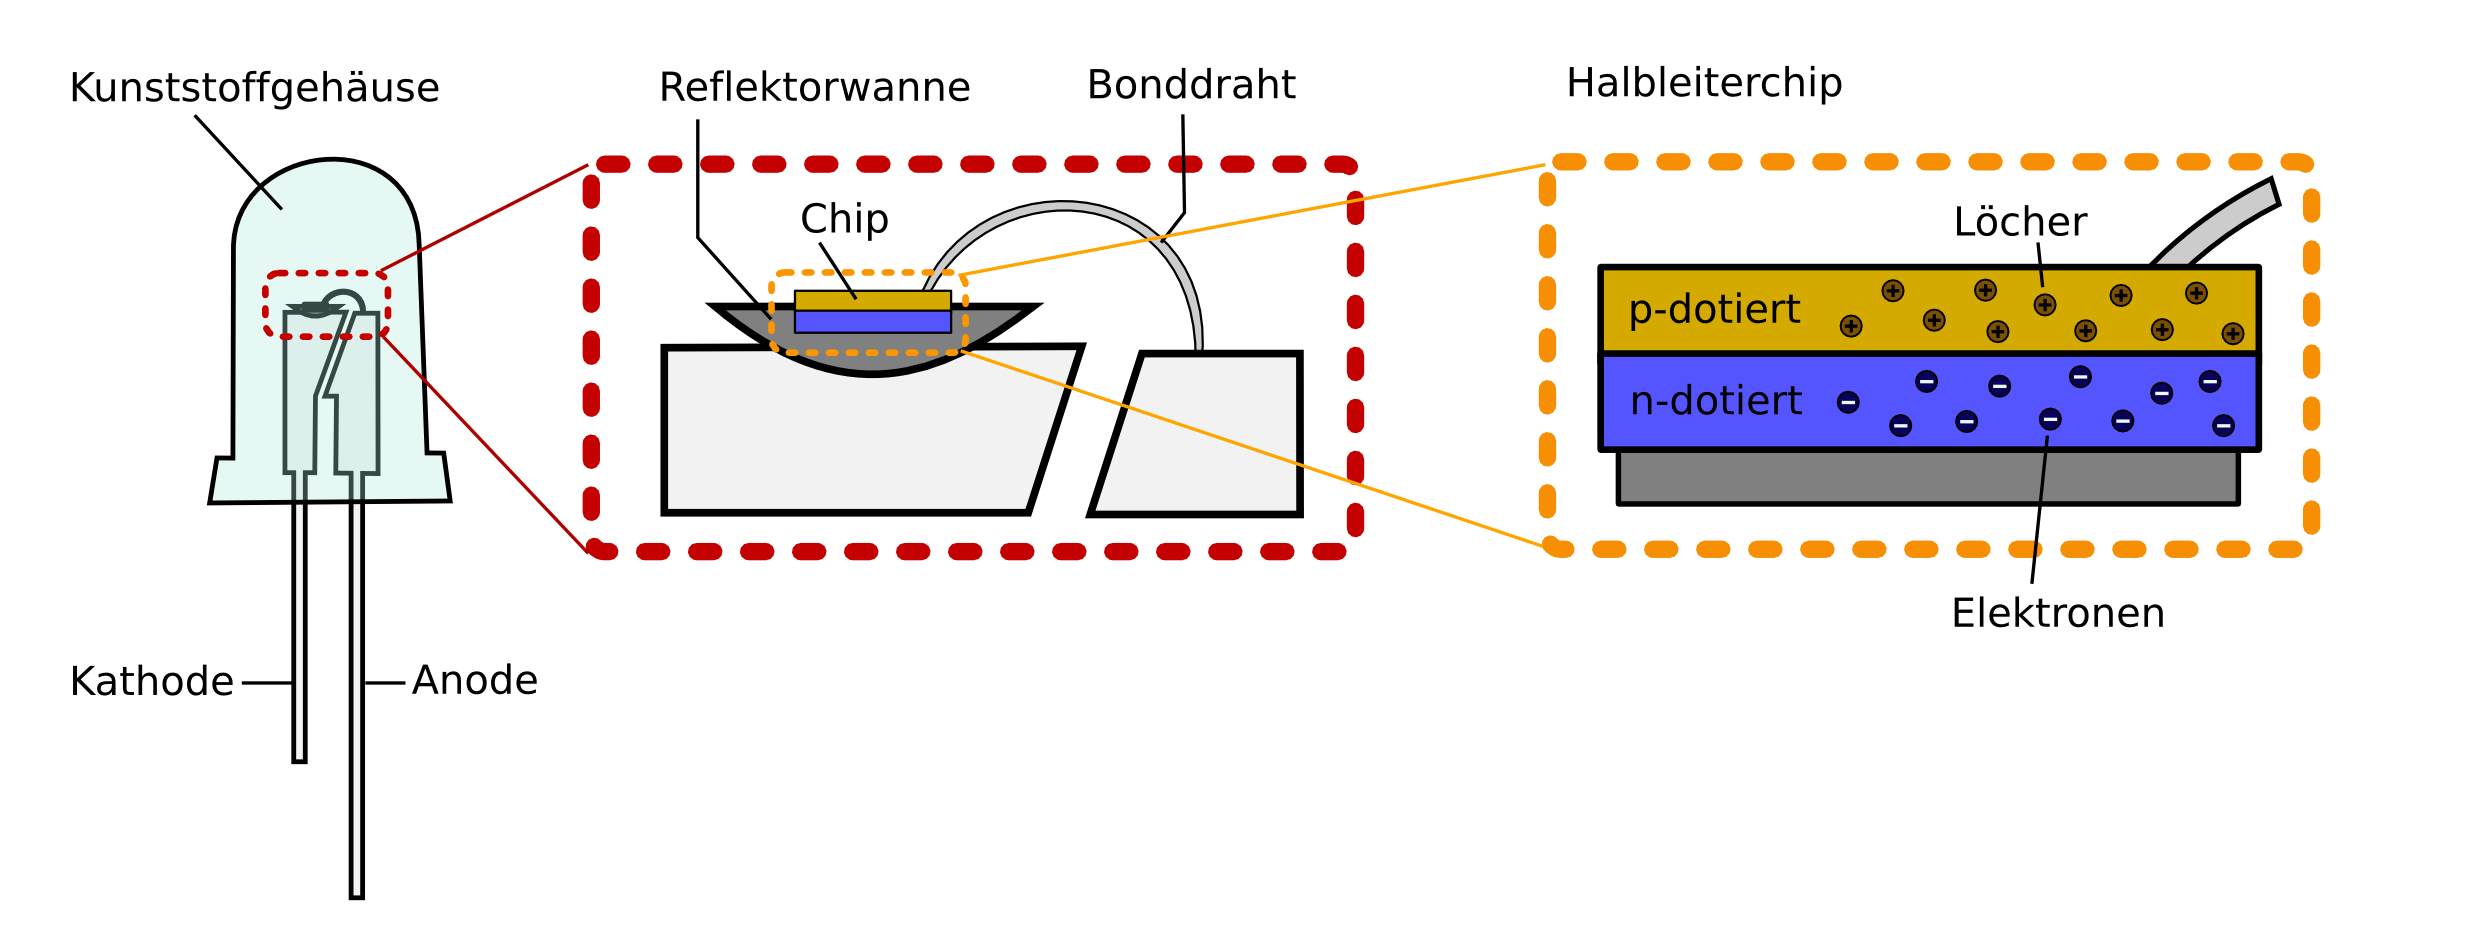
\includegraphics[width=1\textwidth]{ledaufbau.png}
\end{center}
\vspace{-1.5\baselineskip}
\caption{Aufbau einer bedrahteten Leuchtdiode}
\label{LED-Aufbau}
\end{figure}

Da im vorliegenden Projekt nur bedrahtete LEDs als Absorber verwendet wurden, wird im Folgenden nur der Aufbau dieser Leuchtdioden-Bauform dargestellt. Die prinzipielle Funktionsweise ist jedoch bei fast allen Bauarten identisch. Lässt man durch Anode und Kathode der LED einen Strom in Durchlassrichtung fließen, so beginnt der Halbleiter in einer von Material und Dotierung abhängigen Wellenlänge zu strahlen. Für Leuchtdioden im sichtbaren Spektralbereich, wie sie hier verwendet wurden, kommt meist eine Galliumverbindung zum Einsatz.

Das Funktionsprinzip einer LED basiert auf dem Aufbau des Chips, der aus zwei verschieden dotierten Halbleiterschichten besteht. In der p-dotierten Schicht befindet sich ein Überschuss an positiven Ladungsträgern (Löcher), in der n-dotierten Schicht überwiegen negativ geladenen Teilchen (Elektronen). Wird nun ein Strom in Durchlassrichtung an den Chip angelegt, können Elektronen und Löcher am p-n-Übergang rekombinieren. Da sich die Elektronen im n-dotierten Halbleiter im Leitungsband befinden und auf das energetisch niedriger liegende Valenzband der p-dotierten Schicht wechseln, wo sie mit den Löchern rekombinieren, wird ein fester Energiebetrag frei, der in Form eines Photons abgestrahlt wird.

\begin{figure}[ht]
\begin{center}
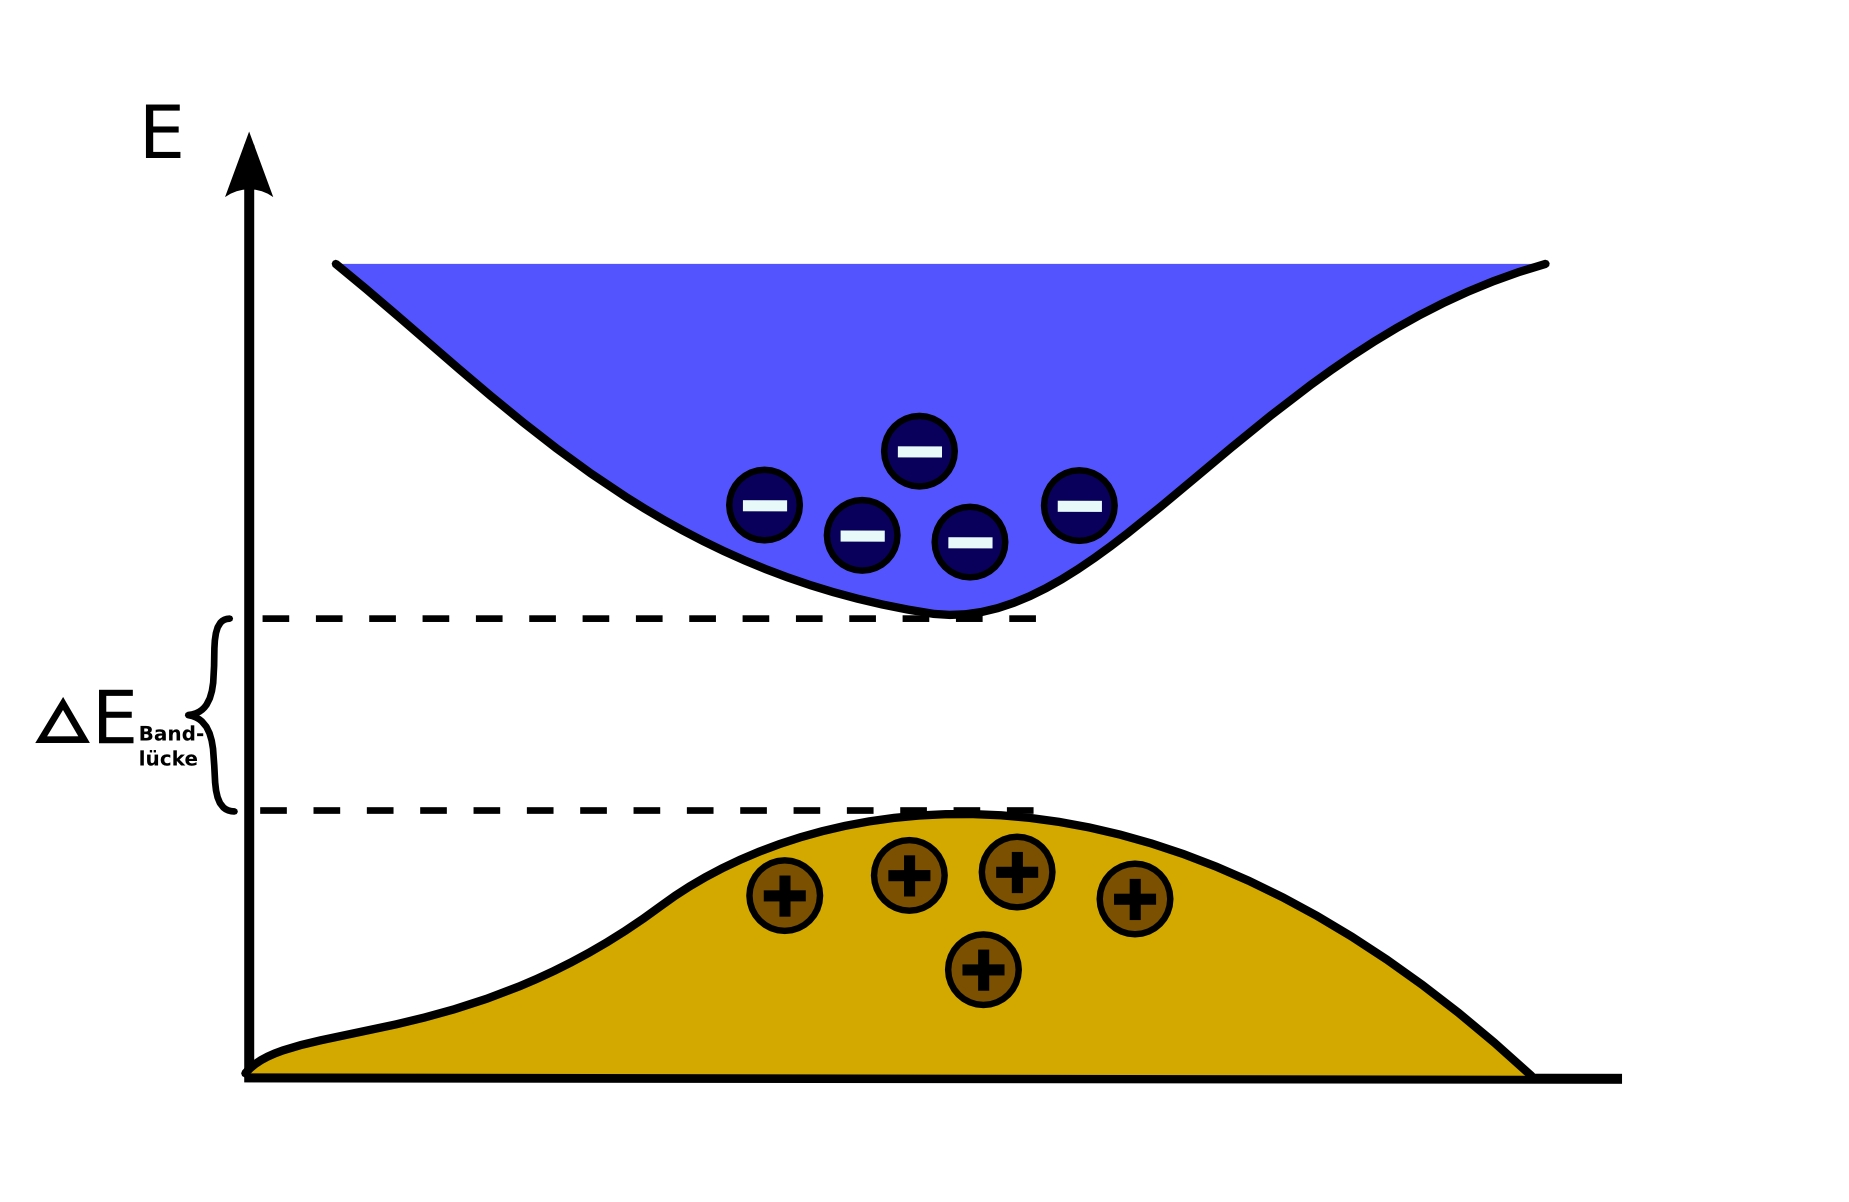
\includegraphics[width=0.8\textwidth]{band.jpg}
\end{center}
\vspace{-1.5\baselineskip}
\caption{B"anderstruktur der Halbleitergrenzschicht}
\label{Baendermodell}
\end{figure}

Die Energie dieses Photons entspricht der Bandlücke zwischen Valenzband und Leitungsband. Somit ergibt sich die Wellenlänge des emittierten Photons wie folgt:
 \[ \lambda = \frac{h \cdot c}{\Delta E_{\text{Bandlücke}}} \]
Dabei bezeichnet $h$ das Plancksche Wirkungsquantum und $c$ die Phasengeschwindigkeit des Lichts.


\subsection{Umkehrung des Effekts - LEDs in der Absorption}
In diesem Versuch sollten jedoch die LEDs nicht als Lichtemitter, sondern als Absorber dienen. Es wurde also versucht, die Funktionsweise der Leuchtdioden umzukehren.

Bei Bestrahlung der LEDs mit Licht kann eine Spannung und ein Strom am Halbleiter abgegriffen werden. Besonderes Interesse gilt der Abhängigkeit dieses Stromes von der Wellenlänge des eingestrahlten Lichtes, je nach Farbe (Emissionswellenlänge) der LED. Da die Leuchtdioden auch in der Absorption wellenlängenabhängig sind, ist es möglich aus mehreren Leuchtdioden, die den gesamten visuellen Spektralbereich abdecken, ein Spektrometer für optische Spektren zu konstruieren.

\subsection{Vergleich von Emissions- und Absorptionsspektren}
\begin{figure}[!b]
\begin{center}
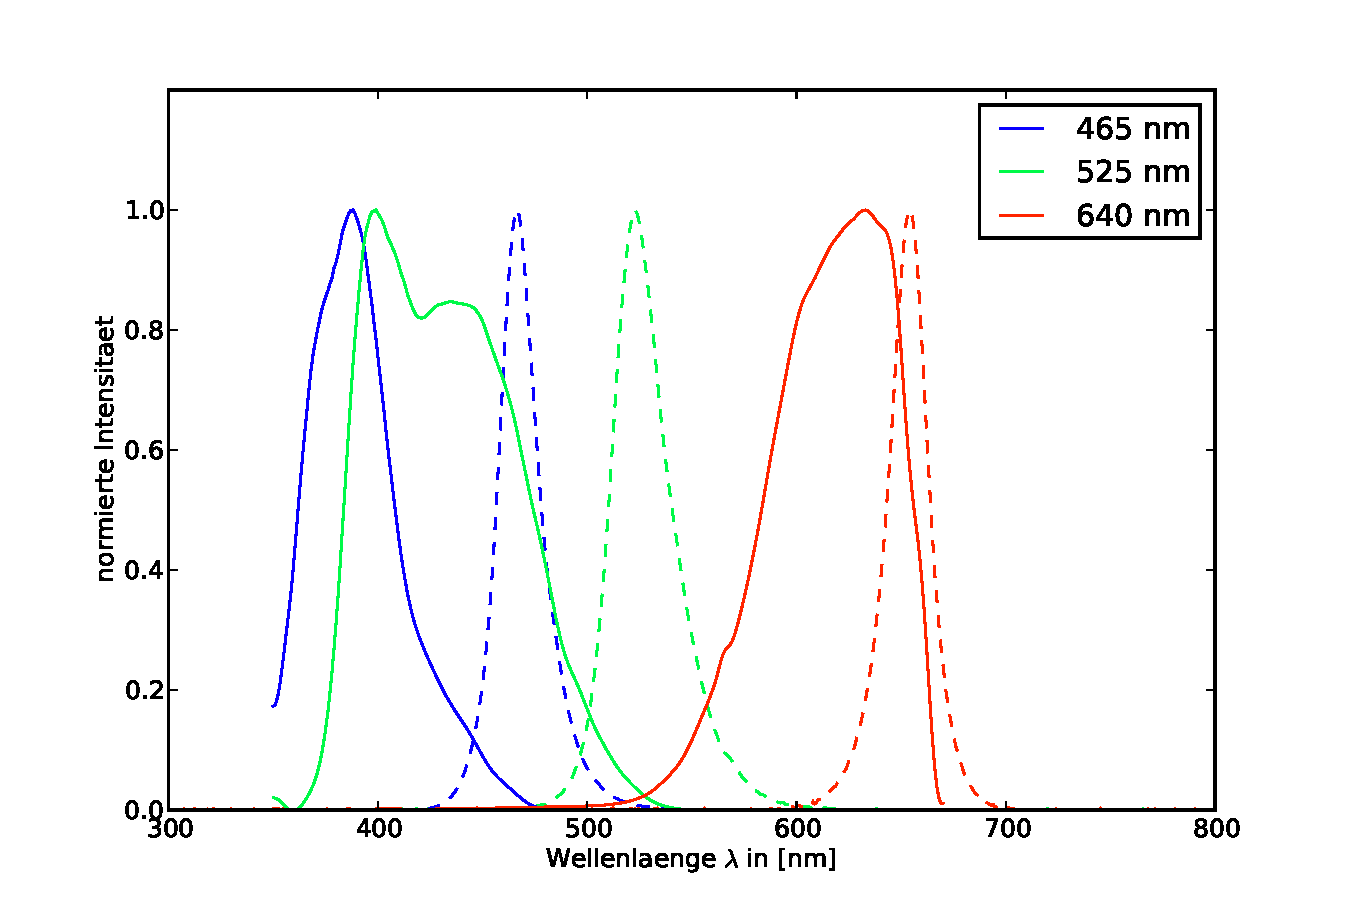
\includegraphics[width=0.9\textwidth]{absorp-emit.pdf}
\end{center}
\vspace{-1.5\baselineskip}
\caption{Absorptions- (durchgezogen) und Emissionsspektren (gestrichelt) verschiedener LEDs}
\label{Absorption und Emission von LEDs}
\end{figure}

Doch was passiert bei der Bestrahlung der LED durch Licht genügender Energie? Treffen Photonen auf die n-p-Grenzschicht des Halbleiterchips, werden dort Elektron-Loch-Paare erzeugt. Durch die Diffusionsspannung wandern die Elektronen in die p-dotierte Schicht, die positiven Löcher in die n-dotierte Zone, wodurch ein Stromfluss entsteht.

%% Vergleich mit den Emissionsspekren
Es stellt sich jedoch die Frage, wie Absorptions- und Emissionsspektrum der Leuchtdiode zusammenh\"angen.
Es ist zu erwarten, dass die LED in der Absorption erst eine Spannung liefert, wenn die Energie der eingestrahlten Photonen mindestens dem Bandlückenabstand entspricht.
Tr\"agt man Absorptions- und Emissionskurve in einem Diagramm auf, ist gut zu erkennen, dass das Absorptionsspektrum gegen\"uber der Emission blauverschoben ist (\hypref{Abb.}{Absorption und Emission von LEDs}) und somit die LED erst auf das eingestrahlte Licht reagiert, wenn die Energie der Bandlücke weit überschritten ist. Quantitativ fällt die Verschiebung $\Delta \lambda$ bei verschiedenen LEDs jedoch unterschiedlich stark aus.
Ein konkreter Zusammenhang zur Wellenlänge der Leuchtdiode oder zum Halbleitermaterial konnte jedoch nicht gefunden werden.



\FloatBarrier
\section{Messung der Absorptionsspektren}


\subsection{Versuchsaufbau}
%subsubsections wohl lieber weglassen, aber zur Meinungsbildung erst noch drinnen gelassen???	
\subsubsection{Lichtquelle} %%Axi
\begin{figure}[!b]
\begin{center}
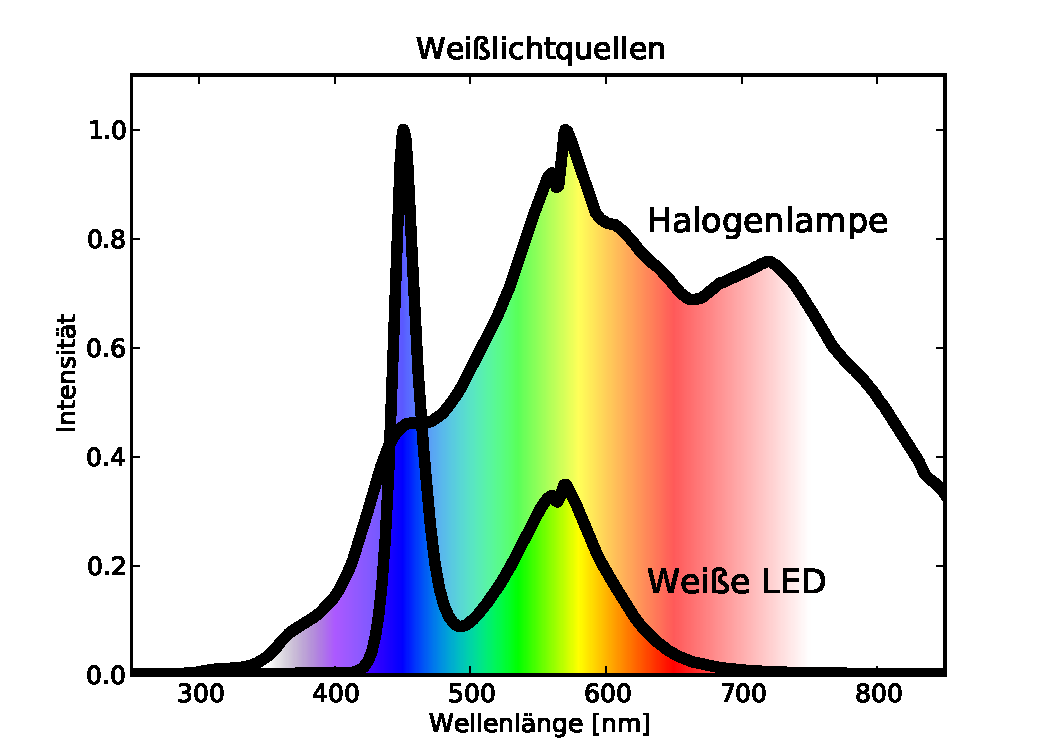
\includegraphics[width=.8\textwidth]{quellspektren.pdf}
\end{center}
\vspace{-1.5\baselineskip}
\caption{Die beiden verwendeten Weißlichtquellen im Vergleich, gemessen mit dem professionellen Spektrometer der Optiker}
\label{fig:lichtquelle}
\end{figure}

Die gew\"ahlte Lichtquelle sollte ein m\"oglichst breites Spektrum mit bekannter Intensit\"atsverteilung aufweisen. Da nur wenige verlässliche Angaben bez\"uglich des jeweiligen Spektrums der Lampen zu finden waren, wurde beschlossen das Spektrum der Lichtquelle mit einem entsprechenden Ger\"at im Institut f\"ur Optik zu ermitteln.

Zun\"achst wurde ein Verbund von vier wei\ss{}en LEDs, die mit einem L\"ufter gek\"uhlt wurden, als Lichtquelle f\"ur die Absorptionsmessung der sp\"ateren Mess-LEDs gew\"ahlt. Als Ergebnis der vier im Quadrat angeordneten LEDs wei\ss{}t deren aufgef\"achertes Spektrum waagrechte, dunkle Streifen auf, die von den Bereichen zwischen den LEDs stammen. Bei der Messung musste deshalb darauf geachtet werden, dass diese Zonen geringerer Intensit\"at zun\"achst durch Defokussieren des Aufbaus mithilfe der eingebauten Linsen verkleinert wurden und anschlie\ss{}end die LEDs die verbleibenden Streifen nicht kreuzten. Dies h\"atte entsprechende Verringerungen in der Intensit\"at des Absorptionsspektrums zur Folge, welche die Messdaten verf\"alschen w\"urden.

\begin{figure}[!b]
\begin{center}
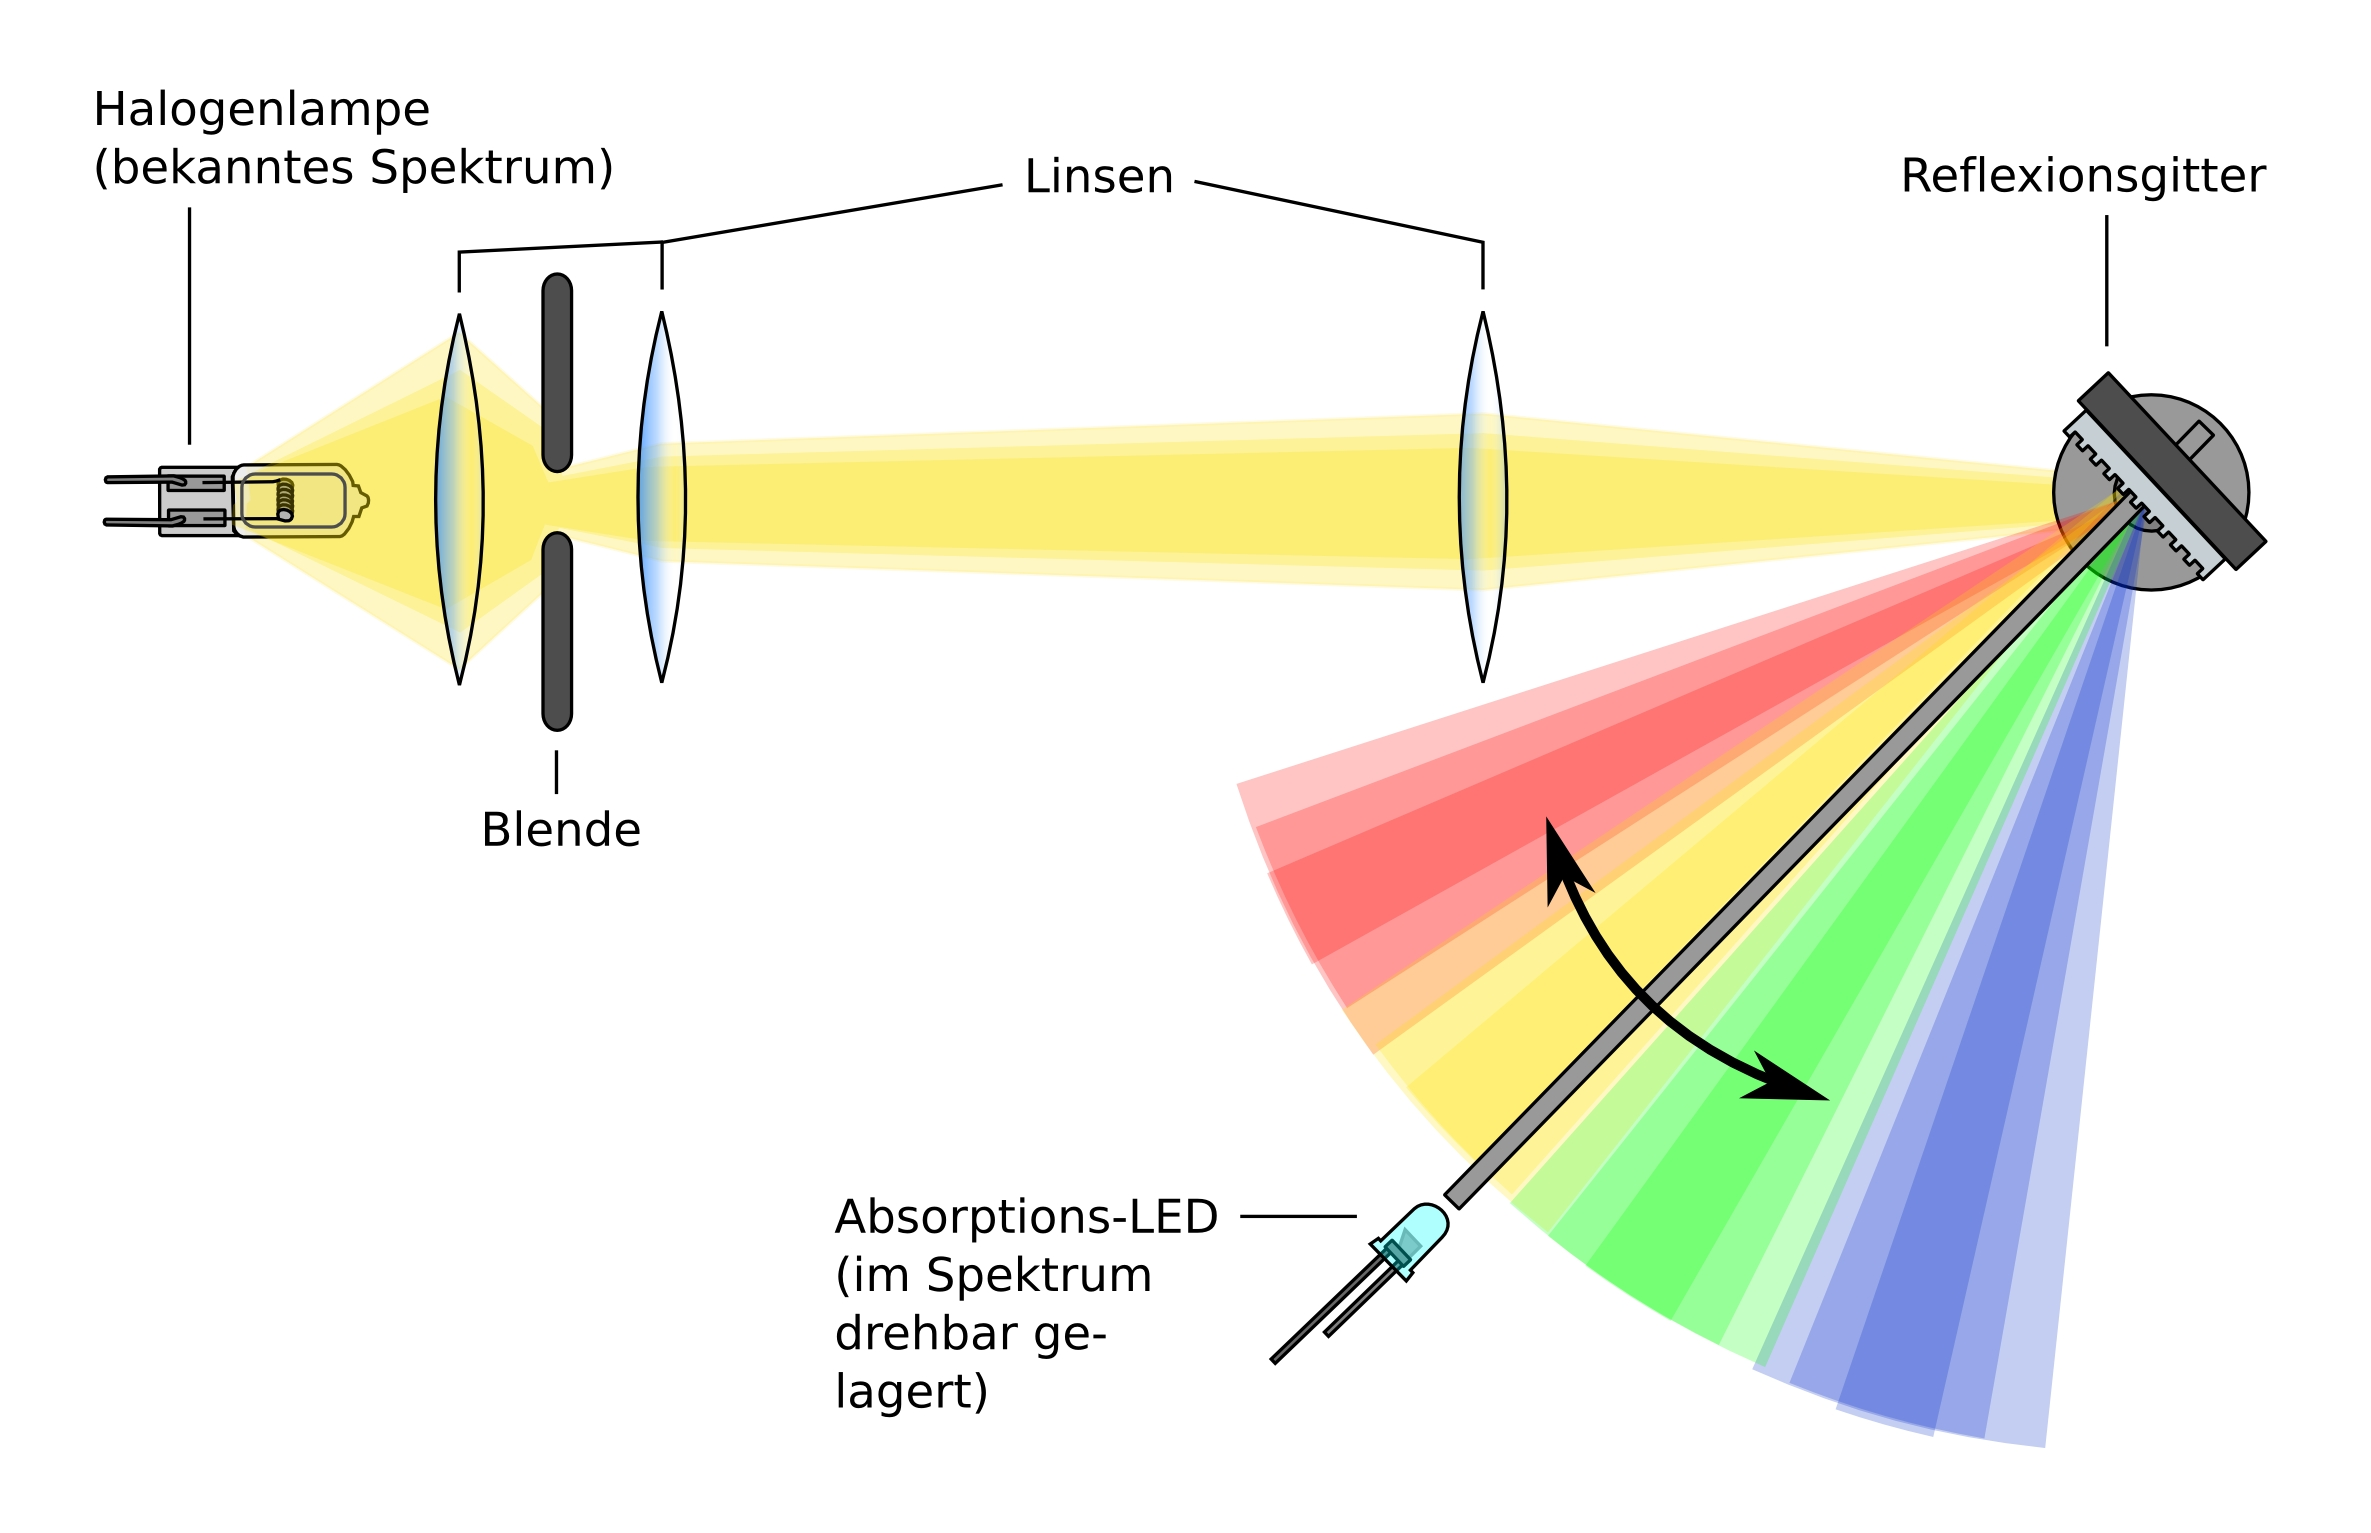
\includegraphics[width=1.\textwidth]{setup.jpg}
\end{center}
\vspace{-1.5\baselineskip}
\caption{Versuchsaufbau schematisch}
\label{Versuchsaufbau}
\end{figure}

Bei der Auswertung wurde festgestellt, dass die Weißlicht-LED-Lichtquelle sehr wenig Intensit\"at im UV-Bereich emittiert (siehe \hypref{Abb.}{fig:lichtquelle}). F\"ur die weiteren Messungen diente deshalb eine 50W Halogenlampe ohne UV-Filter als Lichtquelle. Diese zeigte st\"arkere Intensit\"at im UV-Bereich. Trotz ihrer Nennstromstärke von $4\unit{A}$ brannte die Halogenlampe erst bei $5,3\unit{A}$ durch, so dass wir sie bei $4,7\unit{A}$ betrieben, um möglichst viel Intensität auch noch im UV-Bereich zu erhalten. Da die Halogenlampe durchaus Temperaturen um $200\cel$ erreichen kann, war eine gute Bel\"uftung und ausreichender Abstand hitzeempfindlicher Teile auch hier wichtig.

Im Plot der Weißlichtspektren wird neben der erwarteten Intensitätsverteilung auch eine Charakteristik des Spektrometers der Optiker erkennbar, wie z.B. die Delle bei $564\unit{nm}$. Dies ist ein Problem für spätere Kalibrierungen mit diesem Spektrum, da wir eigentlich davon ausgegangen sind, dass es die Spektren unverfälscht wiedergibt.


\subsubsection{Strahlengang und Messaufbau} %%optischer Strahlengang ist unten eingebaut. Deshalb auch die Idee, die subsubsections weg zu lassen.
Zur Erzeugung eines Spektrums gibt es diverse M\"oglichkeiten. Es stellte sich aber heraus, dass die Verwendung eines Prismas aufgrund der geringen Winkelausdehnung des erzeugten Spektrums f\"ur uns wenig lohnenswert ist. Ebenso mussten wir trotz langen Experimentierens und unter Verwendung verschiedener Linsenanordnungen auch auf ein Transmissionsgitter verzichten, da die Intensit\"at des Spektrums nicht stark genug war. Folglich griffen wir auf ein holographisches Reflexionsgitter zur\"uck, welches mit einer Gitterkonstanten von $d=2400\unit{\text{Linien}/mm}$ ein sehr breites Spektrum erzeugt.%%Gitterkonstante und Winkelausdehnung des Spektrums angeben 2400/mm

\begin{figure}[H]
\begin{center}
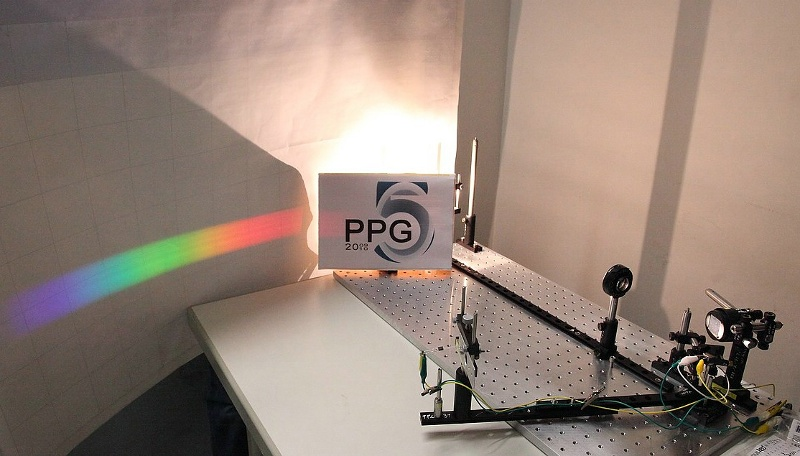
\includegraphics[width=1.\textwidth]{aufbau_spektrum.jpg}
\end{center}
\vspace{-1.5\baselineskip}
\caption{Versuchsaufbau komplett}
\label{fig:aufbau_spektrum}
\end{figure}

%%\subsubsection{Winkelmessung} %%--- Eher "Wellenl\"angenbestimmung" oder dergleichen?! Da wir dadurch ja die momentan gemessene Wellenl\"ange bestimmen m\"ochten
F\"ur die Auswertung der Messdaten ist es von grundlegender Bedeutung zu wissen welcher Wellenl\"ange die gemessene Intensit\"at zuzuordnen ist. Um dies zu erreichen wurde folgendes Vorgehen gew\"ahlt: Durch die Verwendung eines Refelxionsgitters und dessen Justierung derart, dass der Strahlengang in einer zum optischen Tisch parallelen Ebene verl\"auft, l\"asst sich die Wellenl\"ange durch \hypref{Formel}{eq:gitter} leicht in den Winkel $\alpha$ zwischen ein- und ausfallendem Strahl umrechnen.
\begin{equation}
\frac{\lambda}{d} = \sin(\varphi) - \sin(\alpha + \varphi)
\label{eq:gitter}
\end{equation}
Hierbei ist $\varphi = 65,8\degr$ der Drehwinkel des Gitters.

Da ein manuelles Auslesen der Intensit\"at und dessen zugeh\"origem Winkel ein aussichtsloses Unterfangen darstellen w\"urde, benutzten wir ein Drehpotentiometer zur automatischen Auswertung des momentanen Winkels. Dieses wurde so auf dem Tisch positioniert, dass die Drehachse m\"oglichst genau unter dem Mittelpunkt des Gitters ist, also dem Punkt, an welchem sich ein- und ausfallender Strahl treffen. Des Weiteren wurde der Dreharm, an dessen äu\ss{}erstem Ende sich der Halter f\"ur die LEDs befindet, mit der Drehachse verbunden, sodass das Schwenken des Armes den Widerstand des Potentiometers \"andert.

\begin{figure}[ht]
\begin{center}
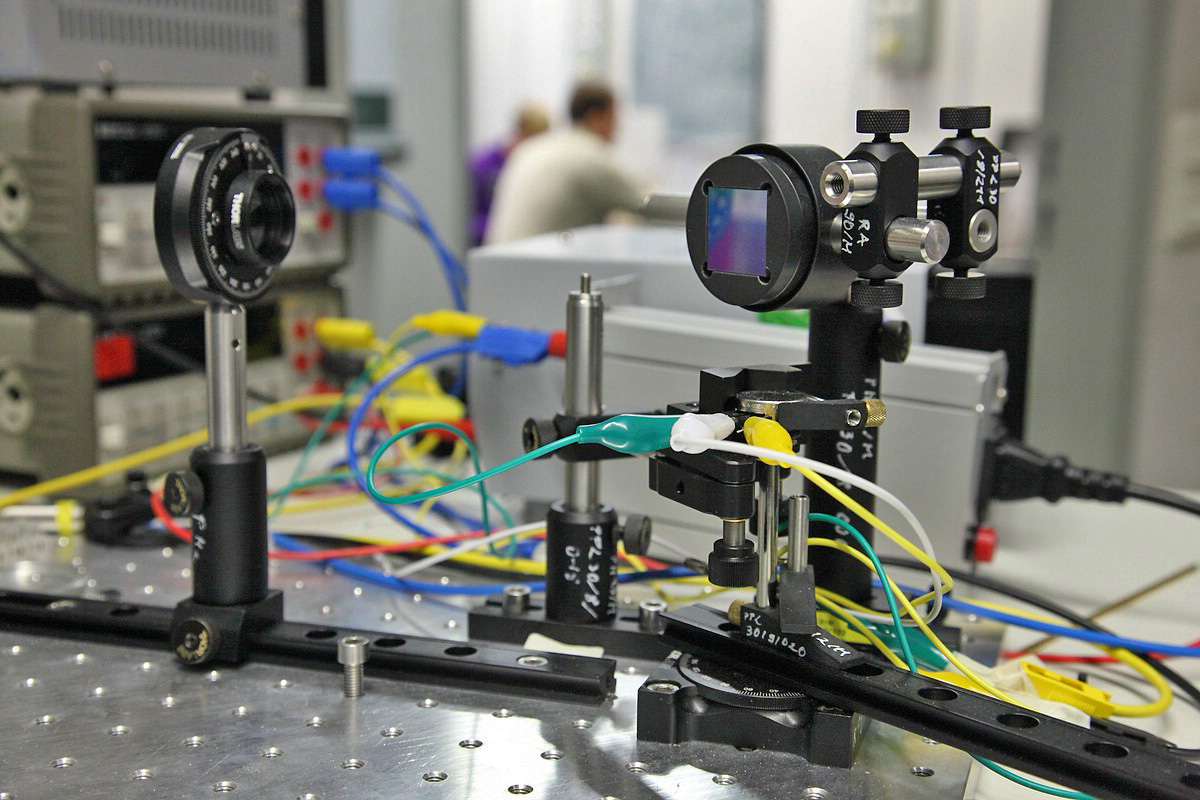
\includegraphics[width=0.8\textwidth]{poti-reflexgitter.jpg}
\end{center}
\vspace{-1.5\baselineskip}
\caption{Das Reflexionsgitter zur Erzeugung des Spektrums und das Potentiometer zur Winkelmessung}
\label{fig:poti-reflexgitter}
\end{figure}

Anschließend wurde in $2^\circ$-Intervallen der Winkel und die Spannung am Potentiometer notiert. Wiederholtes Messen dieser Spannungs-Winkel-Abhängigkeit zeigte eine sehr gute Reproduzierbarkeit. Lediglich beim Wechsel des Drehsinns zeigte sich ein Offset, sodass entschlossen wurde alle Messungen immer mit Drehung im Uhrzeigersinn durchzuführen.

Somit konnten wir die momentane Spannung am Potentiometer auslesen lassen, was uns den Winkel gibt und somit die Wellenlänge berechnen lässt.

\begin{figure}[ht]
\begin{center}
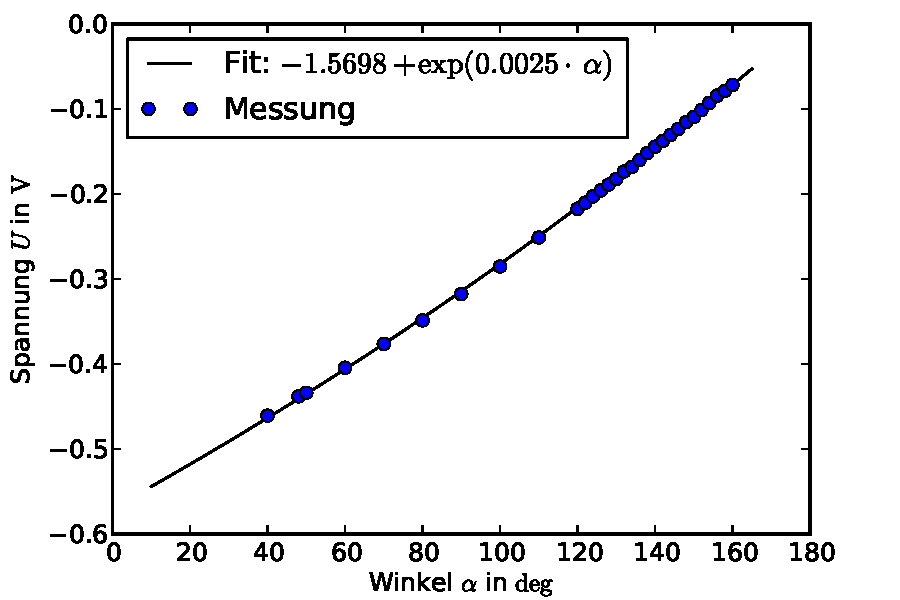
\includegraphics[width=0.8\textwidth]{winkel_spannung.pdf}
\end{center}
\vspace{-1.5\baselineskip}
\caption{Die Potentiometerspannung in Abhängigkeit vom Drehwinkel}
\label{winkel_spannung}
\end{figure}


\FloatBarrier
\subsection{Reduktion der Absorptionskurven}
Aus den aufgenommenen Rohdaten konnten wir mit Hilfe eines hierzu erstellten 500-Zeilen Python Skripts die benötigten Absorptionskurven $I(\lambda)$ berechnen.
Die elektronisch per Computer gemessenen Daten waren Wertepaare von Potentiometerspannung und Absorptions-LED-Spannung über einen Lastwiderstand von $100\unit{k\Omega}$.

Als erster Schritt wurden die Potentiometerspannungen mit Hilfe der in \hypref{Abb.}{winkel_spannung} gefundenen invertierbaren Funktion in Drehwinkel umgerechnet.
Der Winkelbereich des optischen Spektrums lag zwischen $111\degr$ und $158\degr$ (siehe \hypref{Abb.}{Versuchsaufbau}), wo wir die Potentiometercharakteristik sehr gut vermessen hatten.
Als nächstes wurden die Winkel mit Hilfe von \hypref{Gleichung}{eq:gitter} in Wellenlängen umgerechnet. Da der Drehwinkel $\varphi$ des Gitters allerdings schwierig zu messen war, wurde das Interferenzmaximum erster Ordnung, bei dem sich das Gitter wie ein Spiegel verhält, mit aufgezeichnet und aus dessen Lage in der Software der Drehwinkel ausgerechnet. Zusätzlich mussten die Intensitätswerte nach dem Transformationssatz skaliert werden, weil die Wellenlängen nicht gleichmäßig über den Winkelbereich verteilt sind:
\begin{equation}
I(\lambda) = I(\alpha(\lambda)) \;/\; \frac{\dif\lambda}{\dif\alpha}
\end{equation}

\subsubsection{Entfaltung der Absorptionskurven}\label{sec:entfaltung}
Im nächsten Schritt wurde versucht die Absorptionskurven zu entfalten.
Unsere Lichtquelle war natürlich keine Punktquelle und mit dem Linsensystem gelang es auch nicht, die Glühlampe auf einen sehr kleinen Punkt abzubilden.
Infolgedessen würde eine scharfe Spektrallinie als verwaschener Peak erscheinen und von der Absorptions-LED entsprechend aufgenommen werden. Unsere gesamten Absorptionskurven werden somit etwas verbreitert und unscharf gemacht.
Mathematisch gesehen ist das eine Faltung und zwar mit der Punktantwort des optischen Systems als Faltungskern.
Unser Ziel war es also, diese Operation rückgängig zu machen, also eine Entfaltung der Absorptionskurven durchzuführen.

Die Punktantwort des Systems konnte relativ einfach bestimmt werden, indem die Intensitätsverteilung um das nullte Interferenzmaximum herum gemessen wurde.
Die Entfaltung selbst ist jedoch eine relativ schwierige Operation, da nicht unbedingt eine eindeutige Lösung existiert und kleine Fehler im Signal überinterpretiert und zu großen Fehlern in der Lösung führen können.

Somit haben wir verschiedene Algorithmen ausprobiert und auf ihre Tauglichkeit überprüft.
Ein vielversprechender Ansatz war die "`Wiener Deconvolution"'.
Diese nutzt aus, dass die Faltung im Fourierraum einer Multiplikation entspricht, wodurch man zum Entfalten eine Division im Fourierraum durchführen muss.
Zur Unterdrückung von zu starken Rauscheffekten geht noch eine Abschätzung der Fehler im jeweiligen Frequenzbereich mit ein.
Leider mussten wir aber feststellen, dass das Verfahren insgesamt nicht die erwünschten Ergebnisse liefern konnte, vor allem weil die verschiedenen Frequenzterme sich immer auf das ganze Spektrum auswirken.
Das Glätten von Oszillationen an einer Stelle führte gleichzeitig auch zu Verfälschungen an spitzen Peaks.

Der zweite Ansatz führte auf Matrizen.
Da wir ohnehin auf diskretisierten Daten arbeiten, kann man die Faltung auch als Matrix-Multiplikation interpretieren.
Die Entfaltung entspricht dann einer Invertierung.
Die direkte Invertierung ist aber wieder völlig unbrauchbar, da extrem starke Oszillationen entstehen.
In der Tat wären diese eine Lösung des Entfaltungsproblems, nur eben nicht die Gesuchte.

\begin{figure}[H]
\begin{center}
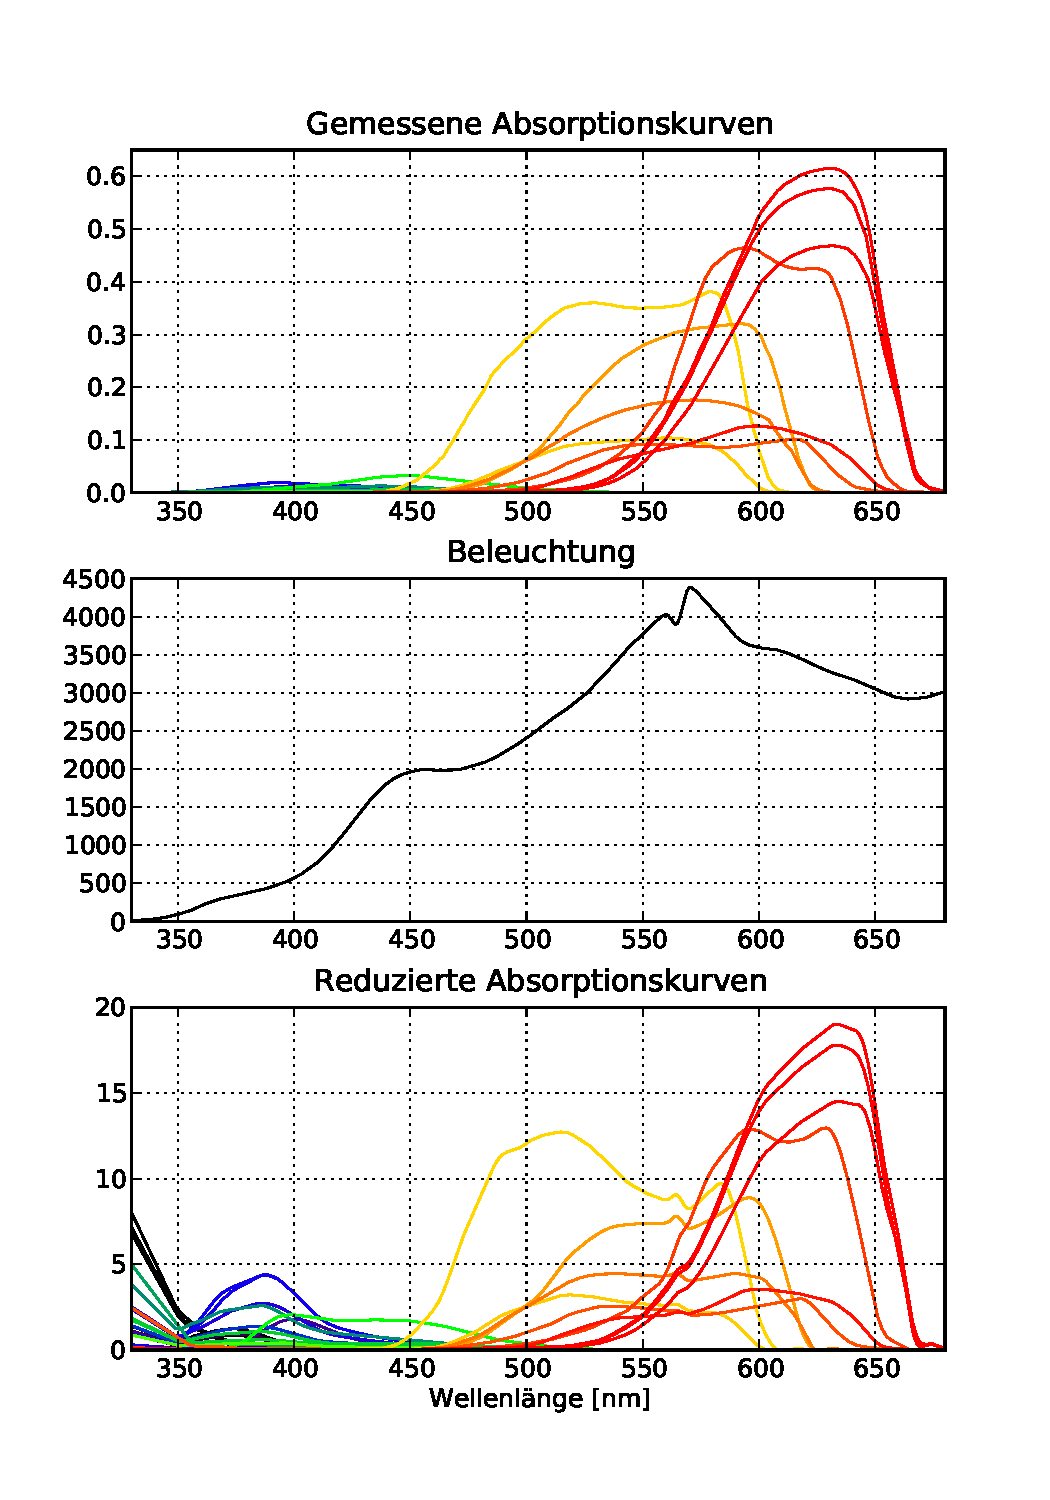
\includegraphics[height=20cm]{spektren_mit_halogen.pdf}
\end{center}
\vspace{-1.5\baselineskip}
\caption{Reduktion der gemessenen LED-Absorptionsspektren}
\label{fig:reduktion}
\end{figure}

Zur Unterdrückung der Oszillationen haben wir nun die Methode der kleinsten Quadrate instrumentalisiert.
Nach dem bekannten Trick an ein Matrixgleichungssystem einfach von links die transponierte Matrix anzumultiplizieren, kann man noch zusätzliche Terme hinzuaddieren, die dann bei der Lösung des Systems mit minimiert werden.
In diesem Fall addiert man die Matrix, welche für jeden $x$-Wert die Krümmung ausrechnet, so dass das System wie folgt aussieht:
\begin{equation}
A\cdot x = b
\qquad\qquad
K = \alpha\cdot
\begin{pmatrix} 
  1 &	-2 &	1 &	&	\\
  &	\ddots&	\ddots&	\ddots&	\\
  &	&	1 &	-2 &	1
\end{pmatrix} 
\qquad
\alpha\in\mathbb{R}
\end{equation}
\begin{equation}
\Rightarrow\qquad
x \approx (A^t A + K^t K)^{-1}\cdot  A^t b
\end{equation}
Hierbei ist $A$ die Faltungsmatrix, die aufgrund der endlichen Faltungsbreite eine Bandstruktur aufweist, $K$ die Krümmungsmatrix mit einstellbarem Vorfaktor $\alpha$, $b$ die gemessene Absorptionskurve und $x$ die Lösung der entfalteten Absorptionskurve.
Die so erzeugten Lösungen erschienen relativ brauchbar.
Anstatt von $K$ wurden auch Matrizen probiert, die auf Terme höherer Ordnung reagieren, was aber zu keinem signifikant besserem Ergebnis geführt hat.
Nachteilig an so einem linearen Verfahren ist natürlich, dass negative Lösungen an einigen Stellen nicht unterdrückt werden können.

Am Ende zeigte sich, dass die Absorptionsspektren im Vergleich zum Faltungskern relativ breit sind.
Der Effekt der Faltung ist also relativ gering wenn man bedenkt, dass dieser auch nur an Stellen auftritt, wo die Funktion gekrümmt ist.
Letztlich wäre es also kein großer Fehler gewesen, die Faltung komplett zu vernachlässigen und die Spektren ohne Entfaltung zu übernehmen.

Zwischen den einzelnen Schritten mussten die Daten für manche Operationen auf ein äquidistantes Gitter gebinnt werden, was einfach mit linearer Interpolation durchgeführt wurde.
Als letzten Schritt wurde berücksichtigt, dass das eingestrahlte Spektrum nicht gleichhell in allen Wellenlängen war.
Die Absorptionskurven wurden nun einfach noch durch die Intensität der jeweiligen Lichtquelle (\hypref{Abb.}{fig:lichtquelle}) geteilt.
Am Rand des Spektralbereichs, wo die Intensität gering war, sieht man daher auch die größten Fehler.
Weiterhin fällt auf, dass die gemessenen Lichtquellen ein bestimmtes Muster enthalten, was bei unseren Messungen aber nicht vorhanden war, und daher invers aufgeprägt wurde.
Dieser Fehler kann fast nur an dem kommerziellen Kalibrations\-spektrometer liegen.

Die fertig reduzierten Absorptions\-spektren sind in \hypref{Abb.}{fig:reduktion} dargestellt.



\FloatBarrier
\section{Bau des Spektrometers}
Im zweiten Teil unseres Projektes konstruierten wir ein funktionsfähiges Gerät, welches die nun bekannten Eigenschaften der Leuchtdioden benutzt, um beliebige Spektren auszumessen und darzustellen.


\subsection{Funktionsprinzip} %Basti
Die am besten geeigneten  Leuchtdioden wurden hierzu nebeneinander auf eine Platine gelötet, die im späteren Messvorgang mit einer unbekannten Lichtquelle beleuchtet werden kann.
Über entsprechende Bauelemente wird das Signal aller 16 Dioden einzeln gemessen, verstärkt und in kurzen Zeitintervallen über die serielle Schnittstelle an den PC gesendet.

Diese Signale stellen aber noch kein Spektrum dar! Schließlich deckt jede einzelne Diode nicht nur einen kleinen Bereich des Spektrums ab, sondern hat eine breite, individuelle Empfindlichkeitskurve, die mit den anderen Kurven überlappt.
Dennoch tragen die Signale genug Information über das gesamte Spektrum, um es in der Software mit einem mathematischen Algorithmus wieder zu rekonstruieren.
Das fertige Spektrum wird dann als Diagramm am Bildschirm des Computers angezeigt.


\subsection{Elektronik}

Um die Photoströme aller 16 LEDs auf möglichst einfache Weise gleichzeitig messen zu können, haben wir in der Elektronikwerkstatt zwei Platinen in Auftrag gegeben (siehe \hypref{Abb.}{fig:electronics}).

\begin{figure}[ht]
\begin{center}
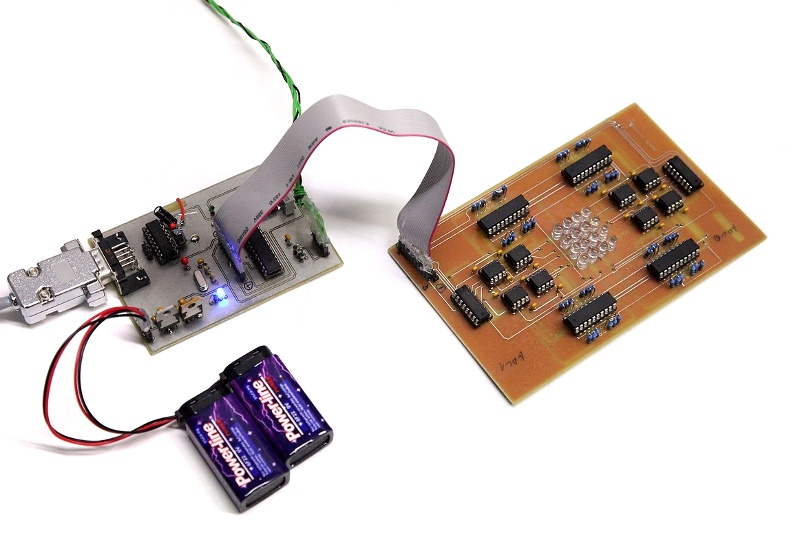
\includegraphics[width=1.\textwidth]{platinen.jpg}
\end{center}
\vspace{-1.5\baselineskip}
\caption{Selbstkonstruierte Elektronik zum Messen der Photoströme der LEDs}
\label{fig:electronics}
\end{figure}

Auf der LED-Platine (größere Platine mir brauner Färbung) befindet sich zentral die Sensor-LED-Matrix. Dieser Aufbau bereitet dabei zwei große Probleme: Durch die große räumliche Ausdehung der Sensor-Matrix ist es schwer sicherzustellen, dass jede Photodiode mit der gleichen Intensität bestrahlt wird, was aber für eine exakte Messung von großer Wichtigkeit ist. Weiterhin erzeugt besonders der von uns verwendete Gehäusetyp eine starke Abhängigkeit bezüglich des Einfallswinkels des zu analysierenden Lichts.

Um die Photoströme der LEDs (typ. $100 \unit{nA}$) in eine messbare Spannung umsetzen zu können, verwenden wir weiterhin für jede Diode einen Transimpedanzverstärker (siehe \hypref{Abb.}{fig:transimp}), welcher im Wesentlichen aus einem Operationsverstärker besteht. 

Die durch den Photostrom hervorgerufene Spannung am Ausgang des Verstärkers ist hierbei äquivalent zur Spannung, die an einem Ohmschen Widerstand abfallen würde.
\begin{equation*}
U_{\text{out}} = R_{\text{Mess}} \cdot I_{\text{Photo}}\,
\end{equation*}
Der große Vorteil dieser aufwendigeren Schaltung gegenüber einer Messung über einen Shunt liegt aber darin, dass der Eingangswiderstand der Operationsverstärker, welcher parallel zur LED anliegt, vernachlässigbar ist. Somit werden die LEDs praktisch kurzgeschlossen, wodurch verhindert wird, dass weitere Phänomene, wie etwa der wellenlängenabhängige Lichtelektrische Effekt
\begin{equation*}
U_{\text{Photo}} = \frac {h \nu - W_{\text{Austritt}}} {e},
\end{equation*}
die Ergebisse verfälschen können. Wir verwenden für alle LEDs einen Messwiderstand $R_{\text{Mess}} = 100 \unit{k \Omega}$.

Um Induktionsströme, die beispielsweise aus dem Stromnetz eingestreut werden können, weitgehend zu vermeiden, sind die Operationsverstärker (8-beinige ICs) auf der Elektronik möglichst dicht um die LEDs platziert worden. Wir verwenden wegen seines geringen Spannungs- sowie Stromrauschens einen OPA 2134, das eher geringe Bandbreiteprodukt ist aufgrund der geringen angestrebten Messwiederholrate (im Bereich von $1 \unit{Hz}$) ausreichend\footnote{\href{http://focus.ti.com/general/docs/lit/getliterature.tsp?genericPartNumber=opa2134&fileType=pdf}{Datenblatt OPA 2134}}. Auf einen Eigenoszillationen verhindernden Rückkopplungs-Kondensator parallel zum Messwiderstand haben wir bewusst verzichtet, da diese bei ersten Tests mit dem Verstärker in keinem signifiakten Maße auftraten. Allerdings könnte diese Einsparung eine Ursache für die instabilen Ergebnisse der Spektrenrekonstruktion darstellen. \\
Für die weitere Verarbeitung der resultierenden Spannungen werden die Ausgänge von jeweils 8 Verstärkern über Multiplexer zu einer Leitung zusammengefasst.

\begin{figure}[H]
\begin{center}
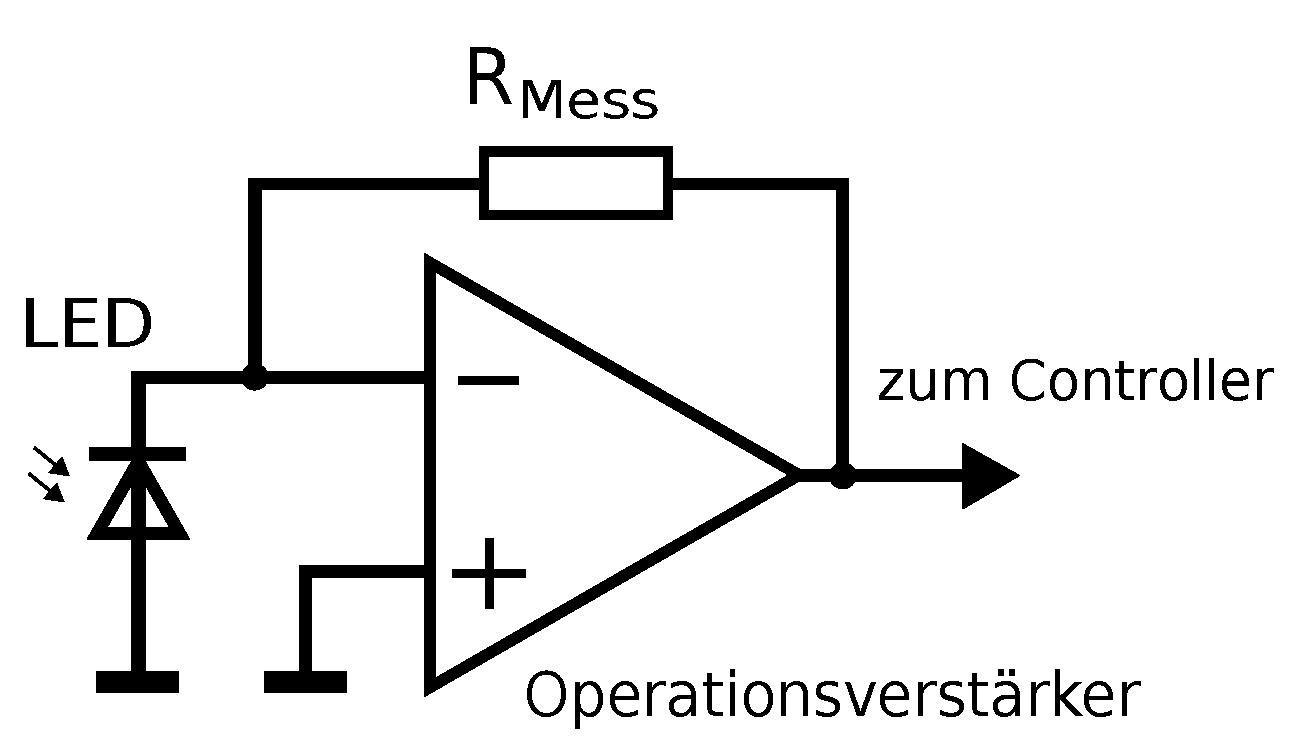
\includegraphics[width=0.5\textwidth]{transimp.pdf}
\end{center}
\vspace{-1.5\baselineskip}
\caption{Transimpedanzverstärker}
\label{fig:transimp}
\end{figure}

Auf der Digitalplatine (kleinere Platine mit grauer Färbung) befindet sich, neben der Spannungsversorgung und einem Pegelwandler für die Kommunikation über die serielle Schnittstelle,  das Herzstück unserer Elektronik, ein in C programmierter Mikrocontroller\footnote{\href{http://www.atmel.com/dyn/resources/prod_documents/doc2486.pdf}{Datenblatt ATmega 8}}.

Die Spannungen $U_{\text{Mess}}$ der LEDs werden über einen integrierten 10-bit Analog-Digital-Converter gemessen, es wird also eine von der Refernzspannung $U_{\text{ref}}$ abhängige Auflösung von $U_{\text{ref}}/1024$ erreicht, wobei wir durch dynamische Anpassung des Messbereichs über Umschalten der Referenzspannung mittels eines Analogschalters Photoströme im Bereich von $10 \unit{nA}$ bis $300 \unit{\mu A}$ messen können. Ein Problem des ADC ist aber der relativ hohe Offsetwert von 17 Einheiten sowie das starke Eigenrauschen, da unsere Messwerte oftmals ebenfalls nur wenige Einheiten betragen. Der Controller übernimmt zudem nach Reskalierung der gemessenen Spannungswerte die Übertragung dieser an den PC. Auf diesem läuft unsere Auswertungssoftware, welche die Rekonstruktion des Spektrums aus den 16 Intensitätswerten übernimmt.

\subsection{Auswertungsprogramm} % Basti
% Software: Berechnung der Spektren mit unserem Gerät
%% Funktionsübersicht und Erklärung der Bedienung
Unsere Auswertungssoftware wurde in Python geschrieben, was den geringsten Programmieraufwand bei solch einer wenig zeitaufwändigen Anwendung versprach.
Im Messbetrieb fordert das Programm vom Controller in manuellen oder regelmäßigen Zeitintervallen von ca. 500\,ms Messwerte an.
Diese bestehen aus einem Vektor mit 16 Einträgen, die bereits auf Ganzzahlen zwischen 0 und 1000 digitalisiert sind.
Jeder dieser Einträge war mit einem Offset von etwa 17 behaftet und hellere Lichtquellen nutzten den Messbereich relativ gut aus, wobei einige der schwächeren Mess-LEDs leider nur Signale von wenigen Einheiten lieferten.

\begin{figure}[H]
\begin{center}
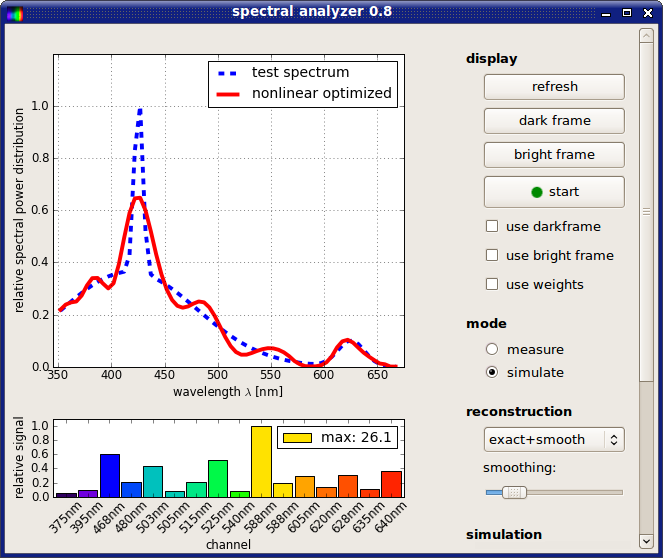
\includegraphics[width=1.\textwidth]{screenshot.png}
\end{center}
\vspace{-1.5\baselineskip}
\caption{Unser Python Programm mit QT-Oberfläche im Simulationsbetrieb}
\label{fig:screenshot}
\end{figure}

Zur Korrektur des Offsets wurde eine Dunkelbild-Funktion integriert.
Dabei nimmt man eine Messung bei abgedeckten Dioden auf.
Die Werte werden zur späteren Verwendung gespeichert und im Messvorgang jeweils von den aktuellen Werten subtrahiert.
Auch eine Helligkeitsanpassung an die tatsächlich gemessenen Werte wurde durchgeführt, indem mit einem Baustrahler Licht eingestrahlt wurde und dessen Spektrum näherungsweise als bekanntes Schwarzkörperspektrum angenommen wurde.
Somit können alle Messwerte noch durch diesen Vergleichswert geteilt werden und veränderte Mess\-charakteristiken der Dioden durch die Elektronik oder sonstige Effekte werden korrigiert.

Zum Test der Algorithmen wurde ein Simulationsmodus eingebaut, der beliebige Spektren würfelt, Messsignale mit einstellbaren Fehlern erzeugt und dann versucht die Spektren wieder zu rekonstruieren.
Damit konnten wir sowohl Funktion und Qualität der Berechnungsmethoden von vornherein abschätzen.

%% Algorithmik zur Auswertung					Basti
\subsubsection{Berechnung des Spektrums}
Die Berechnung eines Spektrums aus den Messwerten ist praktisch das Herzstück unserer Software und bot uns großen Spielraum für mathematische Tüfteleien.
Ein komplettes Spektrum besitzt natürlich unendlich viele Freiheitsgrade, für die wir aber nur 16 Zwangsbedingungen besitzen.
Daher muss man zusätzliche Annahmen in das System stecken, wofür es unzählige Möglichkeiten gibt, von welchen wir eine ganze Reihe getestet haben.

\begin{figure}[H]
\begin{center}
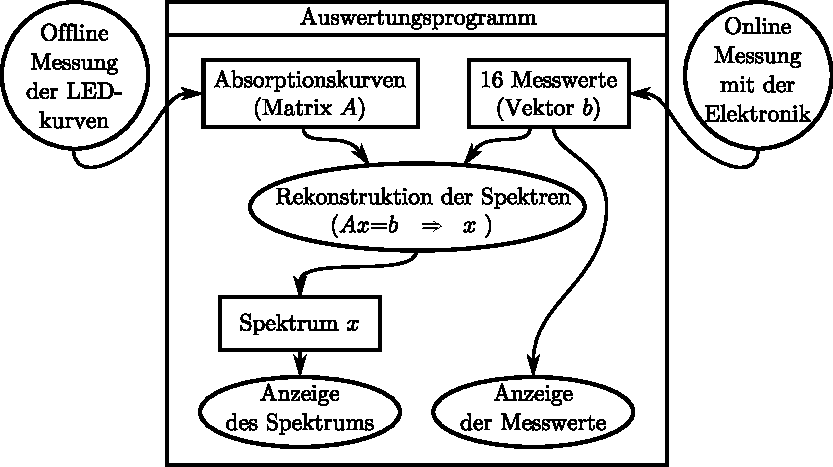
\includegraphics[width=1\textwidth]{programmablauf.pdf}
\end{center}
\vspace{-1.5\baselineskip}
\caption{Skizze des Programmablaufs}
\label{fig:programmablauf}
\end{figure}

Unsere Ausgangsdaten waren also neben dem Vektor der Messwerte $b$ die Absorptionsspektren in Form einer Matrix $A$, gebinnt auf 1\,nm Intervalle zwischen 350 und 670\,nm. Außerdem wissen wir, wie die Messung mathematisch zustande kommt, nämlich:
\begin{equation}
A\cdot x = b
\qquad\qquad
A =
\begin{pmatrix}
\cdots \text{Absorptionskurve 1} \cdots \\
\vdots \\
\cdots \text{Absorptionskurve $n$} \cdots
\end{pmatrix},
\end{equation}
wobei der Vektor $x$ das gesuchte Spektrum ist und die Matrix $A$ nicht quadratisch und somit auch nicht invertierbar ist.
Problematisch ist außerdem, dass die Absorptionskurven in der Matrix sehr breit und im kurzwelligen Bereich sehr ähnlich sind (siehe \hypref{Abb.}{fig:matrixA}).
Der Bereich zwischen 420--470\,nm ist zudem nur schlecht abgedeckt, was an der sogenannten "`Green Gap"' liegen dürfte, also dem Problem, dass es im grünen Emissionsbereich vom 540--580\,nm noch keine effizienten Leuchtdioden gibt.\footnote{\href{http://www.pro-physik.de/Phy/pdfstart.do?mid=3&articleid=51055&recordid=51193}{Physik Journal 1/2010 S. 25f.}}

\begin{figure}[ht]
\begin{center}
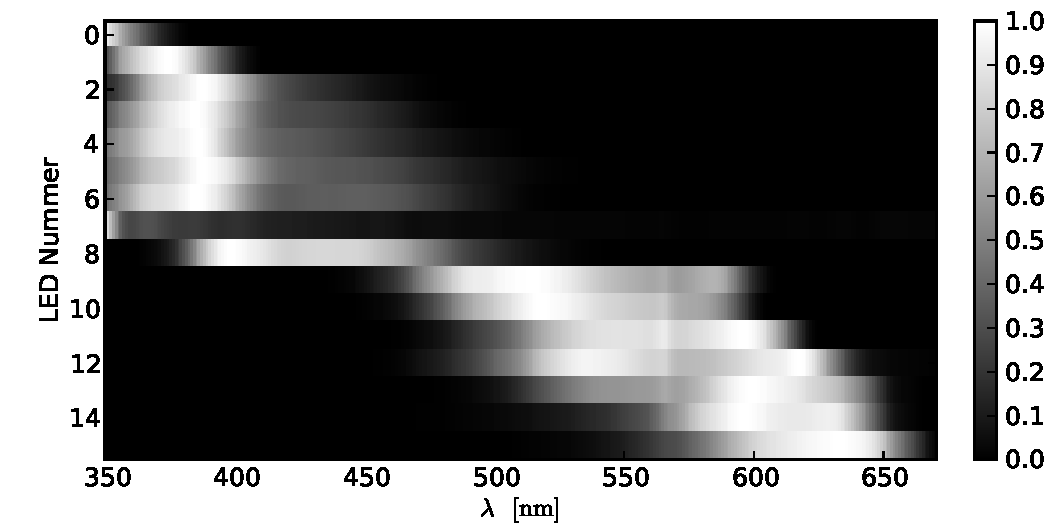
\includegraphics[width=1\textwidth]{matrix_A.pdf}
\end{center}
\vspace{-1.5\baselineskip}
\caption{Bildliche Darstellung der Absorptionskurvenmatrix $A$. Jede Absorptionskurve ist auf 1 normiert.}
\label{fig:matrixA}
\end{figure}

\subsubsection{Exakte Rekonstruktionsalgorithmen}
Die naheliegendste Methode zur Verringerung der Freiheitsgrade ist natürlich die Vergrößerung der Binbreiten, so dass das Spektrum nur noch an 16 unabhängigen Punkten betrachtet wird.
Die Matrix $A$ ist dann tatsächlich invertierbar und liefert immer eine Lösung $x = A^{-1}\cdot b$.
Das Ergebnis ist allerdings völlig unbrauchbar, da die Werte schon bei geringen Messfehlern von unter 1\%, wovon man in der Praxis nur träumen kann, anfangen extrem zu oszillieren und selbst bei fehlerlosen Werten in der Simulation wurde des Spektrum oft nur an sehr wenigen Stellen korrekt wiedergegeben.
Wahrscheinlich ist die Annahme einer konstanten Intensität innerhalb eines Bins einfach schon zu problematisch und die Ähnlichkeit der Absorptionskurven macht die Matrix schon fast singulär.

Die nächste einfache Idee war dann, die Oszillationen zu verhindern, indem von allen Lösungen des fein gebinnten Systems diejenige mit dem geringsten Betragsquadrat genommen wird, also Multiplikation von $b$ mit der Pseudoinversen.
Die Lösung funktioniert schon erstaunlich gut und außerdem effizient, weil die Pseudoinverse nur einmal erzeugt werden muss.
Trotzdem ist das Verfahren aber noch recht anfällig gegenüber Fehlern in den Messwerten und zeigt außerdem wiederkehrende Muster, die von den Absorptionskurven abhängen.

Daher war es ein weiterer Fortschritt nicht die Gesamtnorm des Spektrums, sondern stattdessen die Gesamtkrümmung zu minimieren.
Hierzu benötigt man eine spezielle Lösung $l$ des Systems.
Daraufhin wird eine Basis $L$ des Kerns von $A$ mit der Singulärwertzerlegung erzeugt, dann zusammen mit einer Krümmungsmatrix $K$ wie in \hypref{Abschnitt}{sec:entfaltung} die betragsminimale Lösung des Systems $KL\cdot m = Kl$ und schlussendlich die Lösung $x = l - L\cdot m$.
In Python geht das alles in nur drei Zeilen.
Das Ergebnis ist nochmal besser als die anderen, oszilliert aber auch bei Messfehlern über 1\% recht stark und ist deshalb nicht robust genug.

Andere Ansätze die Lösung in verschiedenste Basen, wie Polynome oder Splines, zu entwickeln waren meistens noch problematischer.
Wir mussten also festhalten, dass die Absorptionskurven einfach zu breit, die Matrix $A$ zu schlecht konditioniert und die Problemstellung zu empfindlich gegenüber Fehlern ist, um exakte Lösungen sinnvoll verwenden zu können.

\subsubsection{Nichtexakte Rekonstruktionsalgorithmen}
Entfernt man sich von der Bedingung, das System exakt zu lösen, so lässt sich beispielsweise die Krümmung der Lösungskurve weiter verringern.
Hierzu kann man die Summe aus Abstandsquadraten zu den Messwerten und der Krümmung der Lösungskurve minimieren und beide Aspekte variabel gewichten.
Die Lösung gewinnt man dann mit
\begin{equation}
x = (A^tA+\beta\cdot K^tK)^{-1}\cdot A^t\,b
\qquad\qquad
\beta\in\mathbb{R} \ ,
\end{equation}
mit der bekannten Krümmungsmatrix $K$ und einem Parameter $\beta$, den man zur Laufzeit anpassen kann.
Bei kleinem $\beta$ und mittelgroßer Binzahl zeigt dieses Verfahren, dass es numerisch nicht unbegrenzt stabil ist.
Wir haben es deshalb mit einem mathematisch äquivalenten Singulärwertverfahren ersetzt.
Durch den variablen Parameter war dieses Verfahren schon sehr universell einsetzbar, da man die Glättung an die Fehlerrate der Messwerte anpassen konnte und so immer ein vernünftiges Signal erhielt.

Weitere Verbesserungen konnten wir nur erreichen, indem wir uns von den linearen Matrizenverfahren trennten.
Viele Ungenauigkeiten und Oszillationen in der Lösungskurve können nämlich verringert werden, wenn die Zusatzbedingung nichtnegativer Intensitätswerte mit beachtet wird.
Unser Ansatz bestand nun einfach darin, eine Zielfunktion zu definieren, welche sowohl die Abstände vom Lösungsvektor, als auch die Krümmung sowie die negativen Werte gewichtet und quadratisch zusammenaddiert.
Diese Funktion wird an einen Minimierungsalgorithmus übergeben, der die optimale Lösung sucht.
Prinzipbedingt braucht dieses Verfahren erheblich mehr Rechenzeit als die anderen, weil die Lösung sehr oft neu ausgerechnet werden muss bis die Konvergenz erreicht ist.
In \hypref{Abb.}{fig:screenshot} wird dieses Verfahren verwendet und man sieht, dass das Originalspektrum bis auf kleinere Oszillationen schon recht gut erreicht wird.
Auch wenn die Möglichkeiten zur Verbesserung noch groß sind, haben wir es vorerst bei diesem Verfahren belassen.

Für spezielle Lichtquellen lohnt es sich außerdem noch mehr Informatio\-nen aus dem Spektrum zu holen.
Von annähernd schwarzen Strahlern lässt sich mit dem Spektrometer die Effektivtemperatur mit einem passenden Schwarz\-körperspektrum ermitteln.
In diesem Modus fittet der Computer ein Planck-Spektrum $I(\lambda)$ mit den beiden Parametern Temperatur und Skalierungsfaktor auf die Messdaten, so dass der Fehler
\begin{equation}
\left(
A\cdot I(\lambda) - b
\right)^2
\end{equation}
minimal wird.
Zur Vermessung von monochromatischen Strahlern haben wird das gleiche mit einer Gaußkurve implementiert.



\section{Fazit}
Zum Ende des Projekts gelang es, ein funktionsfähiges Spektrometer im optischen Bereich zu konstruieren, das vor allem bei Quellen mit schwarzkörperähnlicher Abstrahlcharakteristik gute Resultate lieferte. Für diese Quellen konnte sogar die Farbtemperatur bestimmt werden. Dabei ist noch hervorzuheben, dass die Auswertung quasi „on-the-fly“, d.h. simultan zum Messen, erfolgte.
Verbesserungswürdig ist neben der relativ großen Fehleranfälligkeit noch der Algorithmus, den die Auswertungssoftware zum Berechnen des Spektrums benutzt. Außerdem könnte, zum Beispiel durch einen Neuaufbau mit SMD-Bauteilen, die gegenwärtig recht große Abhängigkeit vom Einstrahlwinkel reduziert werden. Diese Änderungen und weitere Verbesserungen werden in einer Weiterführung des Projekts am Physikalischen Institut III noch implementiert werden.
\end{document}

